% =====================================================================
%  Drop-in section for main_v11.tex
%  "Functional validation of the signed-XOR motif in a spiking model"
%
%  Usage:
%   1. Place the three figures (exp1_rasters.png, exp2_pv_sweep.png,
%      exp3_graded_error.png) from results/ next to the .tex, or in a
%      figures/ directory and adjust the \includegraphics paths.
%   2. Add  % =====================================================================
%  Drop-in section for main_v11.tex
%  "Functional validation of the signed-XOR motif in a spiking model"
%
%  Usage:
%   1. Place the three figures (exp1_rasters.png, exp2_pv_sweep.png,
%      exp3_graded_error.png) from results/ next to the .tex, or in a
%      figures/ directory and adjust the \includegraphics paths.
%   2. Add  % =====================================================================
%  Drop-in section for main_v11.tex
%  "Functional validation of the signed-XOR motif in a spiking model"
%
%  Usage:
%   1. Place the three figures (exp1_rasters.png, exp2_pv_sweep.png,
%      exp3_graded_error.png) from results/ next to the .tex, or in a
%      figures/ directory and adjust the \includegraphics paths.
%   2. Add  % =====================================================================
%  Drop-in section for main_v11.tex
%  "Functional validation of the signed-XOR motif in a spiking model"
%
%  Usage:
%   1. Place the three figures (exp1_rasters.png, exp2_pv_sweep.png,
%      exp3_graded_error.png) from results/ next to the .tex, or in a
%      figures/ directory and adjust the \includegraphics paths.
%   2. Add  \input{functional_validation}  after Section~\ref{sec:functional}
%      (the autoencoder reservoir experiment) and before the synthesis
%      Section~\ref{sec:synthesis}, OR keep it as its own top-level section
%      just before "Proposed experimental validation plan".
%   3. The block reuses the paper's existing environments
%      (prediction, conjecture, remark) and citation keys
%      (Billeh2020, Cardin2009, Atallah2012) -- no new packages needed.
%   4. Replace OWNER/REPO in the \url below with the public repository.
%
%  All numbers below are the actual output of the released code
%  (commit-pinned in results/*.json). Re-running run_all.py reproduces them.
% =====================================================================

\section{Functional validation: a spiking signed-XOR motif}
\label{sec:spiking}

The structural analysis (Sections~\ref{sec:scope}--\ref{sec:synthesis}) and
the reservoir experiment (Section~\ref{sec:functional}) treat the Allen V1
model as a static, signed graph; as stated in the Scope, they do not model
firing rates or spike timing, and a full functional characterisation
``requires spiking simulation with realistic rates.'' This section supplies
the minimal such characterisation for the \emph{isolated} eight-neuron motif.
The aim is narrow and deliberate: not to simulate V1, but to test whether the
signed-XOR computation defined in Section~\ref{sec:motif} actually emerges
from leaky integrate-and-fire (LIF) dynamics with mouse-V1 cell-type time
constants, and to convert the firing-rate caveat raised in the Abstract and in
Section~\ref{sec:scope} into a concrete, falsifiable prediction.

\subsection{Model}
\label{sec:spiking_model}

We instantiate the eight roles of Section~\ref{sec:motif}
($E_1, E_3$ inputs; $E_2, E_4$ latents; $\mathrm{INH}$ pivot;
$\mathrm{XOR}$ comparator; $F^+, F^-$ signed-error outputs) as current-based
LIF neurons in Brian2 \citep{Stimberg2019}, one neuron per role, wired with
the twelve directed edges of the motif. Membrane time constants are assigned
per Allen V1 cell type: thalamo-recipient inputs as \texttt{e4other}
($\tau_m=12$~ms), latents and comparator as \texttt{e23Cux2}
($\tau_m=15$~ms), and the inhibitory pivot as a fast-spiking
\texttt{i4Pvalb} interneuron ($\tau_m=6$~ms), reflecting the empirically
established $2$--$3\times$ faster membrane dynamics of parvalbumin cells
\citep{Cardin2009,Atallah2012}. The pivot implements the dual role argued for
in Section~\ref{sec:sparse_op}: it is wired as a \emph{coincidence detector},
firing only when both inputs are simultaneously active, and its veto of the
two latents is what realises the exclusive-or. The $F^+$ and $F^-$ neurons are
in turn coincidence detectors on (latent, comparator) pairs, so that they read
out the \emph{sign} of the mismatch. Each trial drives the active input(s) for
$100$~ms; a role is scored ``active'' if it emits $\geq 2$ spikes. Full
parameters, the synaptic weight matrix, and the integration scheme are in the
released code (Section~\ref{sec:availability}); the simulation uses Brian2's
pure-NumPy code-generation target and runs in seconds on a laptop under WSL.

\subsection{Result 1: the motif computes the signed-XOR truth table}
\label{sec:spiking_truth}

Driving the two inputs through all four binary conditions reproduces the
signed-XOR truth table of Section~\ref{sec:motif} deterministically
(Table~\ref{tab:spiking_truth}, Figure~\ref{fig:spiking_rasters}).
When the two inputs agree ($S_1=S_2$) the circuit rests in homeostasis with no
error signal: the silent case $(0,0)$ produces no spikes anywhere, and the
matched-active case $(1,1)$ drives the pivot ($8$ spikes) which vetoes both
latents, so the comparator and both error neurons stay silent. When the inputs
disagree, the comparator fires ($4$ spikes in both mismatch cases) and exactly
one error channel responds: the under-shoot case $(1,0)$ activates $F^+$
($3$ spikes, $F^-$ silent), the appropriate driver of potentiation, while the
over-shoot case $(0,1)$ activates $F^-$ ($7$ spikes, $F^+$ silent), the driver
of depression. The signed-error logic
$F^+ = \max(0, x-r)$, $F^- = \max(0, r-x)$ of Section~\ref{sec:dynamic} thus
holds at the level of spikes, not only in the rate abstraction.

\begin{table}[H]
\centering
\small
\begin{tabular}{cc cccccccc c}
\toprule
$S_1$ & $S_2$ & $E_1$ & $E_3$ & $E_2$ & $E_4$ & INH & XOR & $F^+$ & $F^-$ & interpretation \\
\midrule
0 & 0 & 0 & 0 & 0 & 0 & 0 & 0 & 0 & 0 & homeostasis (no error) \\
1 & 0 & 5 & 0 & 5 & 0 & 0 & 4 & 3 & 0 & under-shoot $\rightarrow$ LTP ($F^+$) \\
0 & 1 & 0 & 5 & 0 & 5 & 0 & 4 & 0 & 7 & over-shoot $\rightarrow$ LTD ($F^-$) \\
1 & 1 & 5 & 5 & 0 & 0 & 8 & 0 & 0 & 0 & homeostasis (matched) \\
\bottomrule
\end{tabular}
\caption{Spike counts per role over a $100$~ms trial for each input
condition. Entries are exact spike counts; a role is read out as active at
$\geq 2$ spikes. The comparator (XOR) is active iff the inputs differ, and the
two error channels $F^+/F^-$ partition the two mismatch directions. The table
is reproduced deterministically; under $20$~Hz Poisson background noise (25
random seeds) the full four-row table is recovered on $88\%$ of trials.}
\label{tab:spiking_truth}
\end{table}

\begin{figure}[H]
\centering
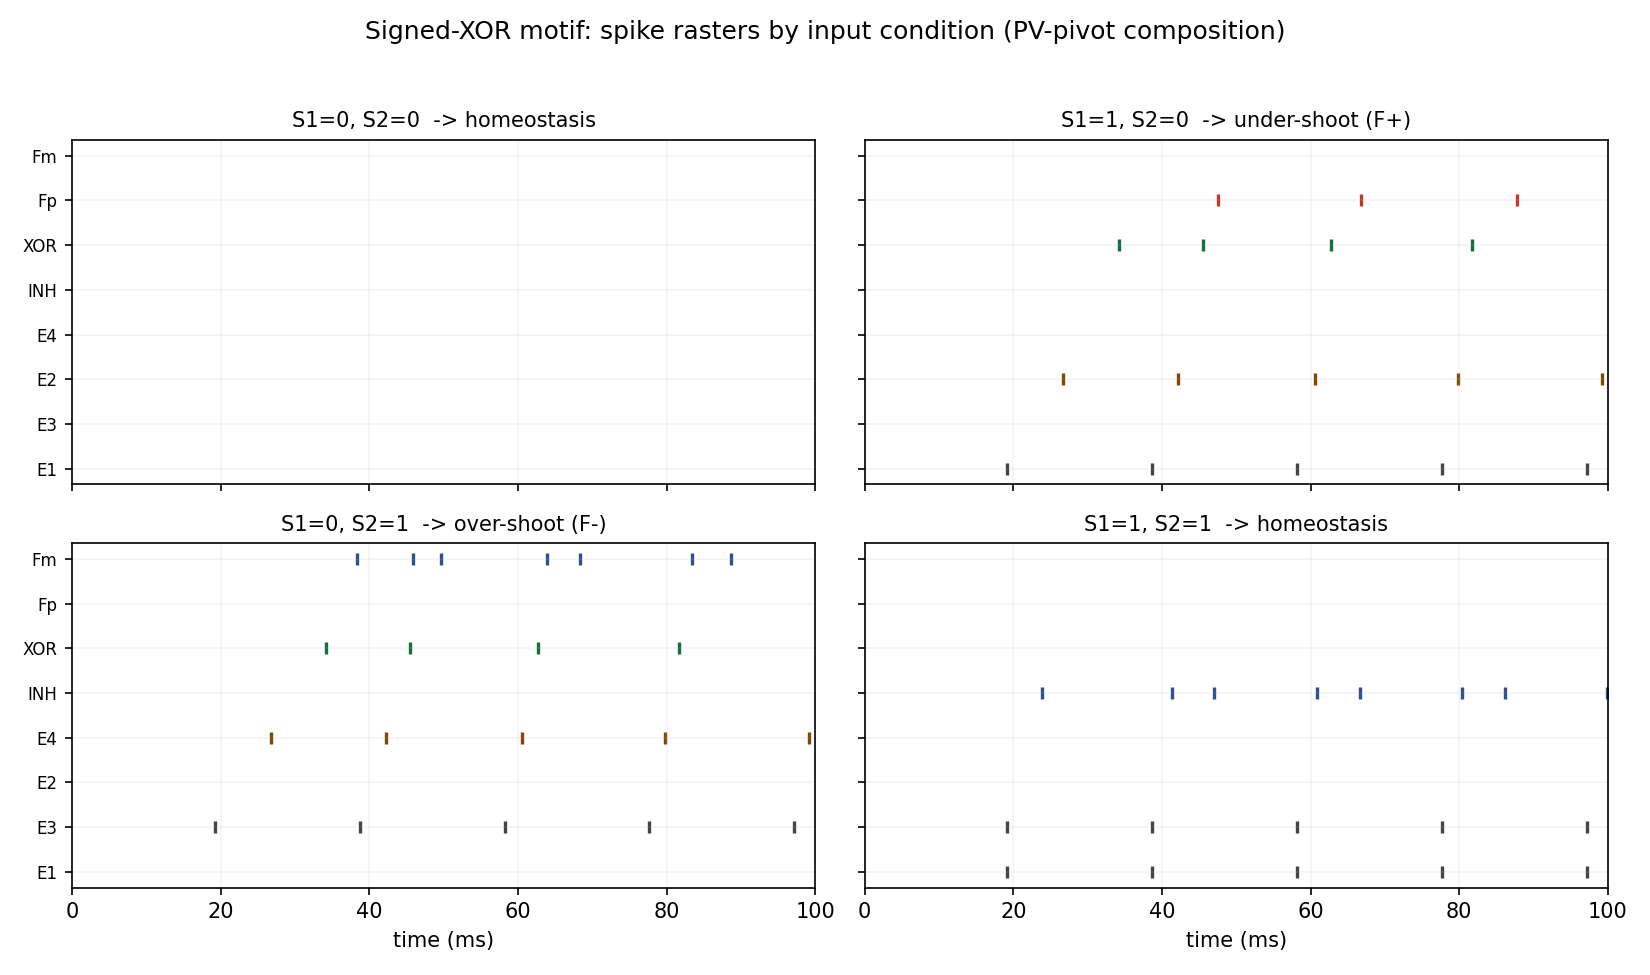
\includegraphics[width=\textwidth]{exp1_rasters.png}
\caption{Spike rasters of the eight motif neurons for the four input
conditions. The inhibitory pivot (INH) fires only when both inputs are
co-active $(1,1)$ and silences the latents; the comparator (XOR) fires only on
mismatch; $F^+$ and $F^-$ each respond to exactly one mismatch direction.}
\label{fig:spiking_rasters}
\end{figure}

\subsection{Result 2: fast-spiking inhibition is required}
\label{sec:spiking_pv}

The coincidence/veto logic of the pivot depends on its membrane integration
window being short relative to the synaptic time scale: a slow pivot integrates
a single input up to threshold and fires spuriously, destroying the exclusive-
or. We tested this directly by sweeping the pivot's membrane time constant
$\tau_m^{\mathrm{INH}}$ from $4$ to $15$~ms while holding everything else fixed,
scoring the full truth table over 15 noisy seeds per value
(Figure~\ref{fig:spiking_pv}). The circuit succeeds on $100\%$ of trials for
$\tau_m^{\mathrm{INH}} \in [6,7]$~ms (fast-spiking, PV-like), degrades through
$\tau_m^{\mathrm{INH}}=8$~ms ($60\%$), and fails completely
($0\%$) for $\tau_m^{\mathrm{INH}} \geq 9$~ms --- i.e.\ at the membrane time
constants of pyramidal ($\sim12$--$15$~ms) or somatostatin/Htr3a interneurons
($\sim10$--$12$~ms). Consistently, instantiating the pivot with the
\texttt{i4Pvalb} cell type yields a working circuit, whereas instantiating it
with the rank-1 empirical \texttt{i4Sst} pivot reported in
Section~\ref{sec:weight_stats} does \emph{not}, at otherwise identical
parameters.

\begin{figure}[H]
\centering
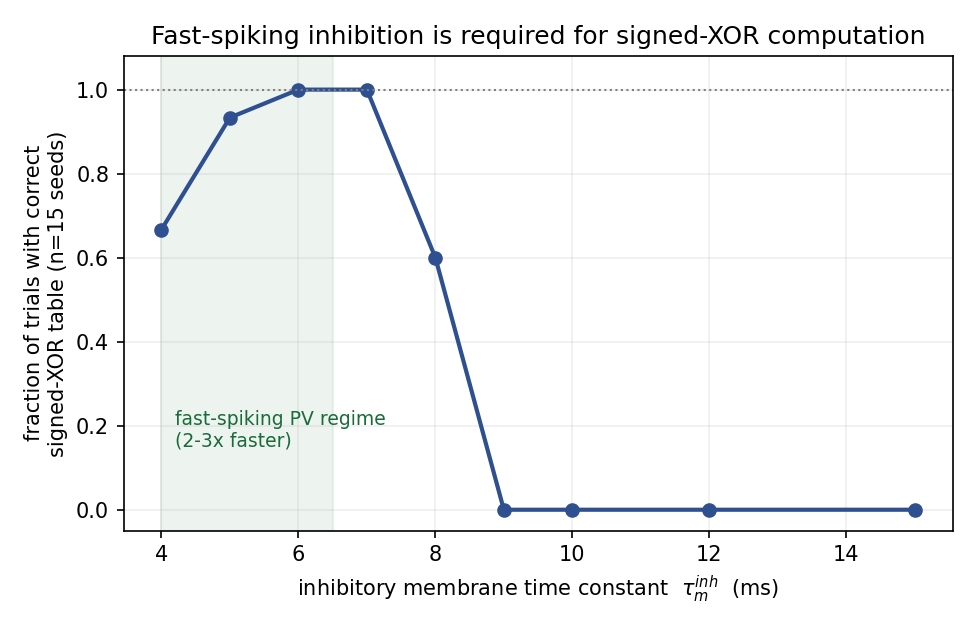
\includegraphics[width=0.78\textwidth]{exp2_pv_sweep.png}
\caption{Truth-table success rate (15 noisy seeds per point) as a function of
the inhibitory pivot's membrane time constant. The functional window
($100\%$ success) is confined to the fast-spiking, parvalbumin-like regime
($\tau_m \leq 7$~ms); the computation collapses at pyramidal and
Sst/Htr3a-like time constants.}
\label{fig:spiking_pv}
\end{figure}

This turns the firing-rate caveat of the Abstract and Section~\ref{sec:scope}
into a sharp, testable claim. The structural analysis is cell-type-agnostic
about which inhibitory subtype occupies the pivot; the dynamics are not.

\begin{prediction}{Fast-spiking pivot requirement}{pv}
A signed-XOR motif instance is \emph{functional} (computes the exclusive-or and
its signed error) only if its inhibitory pivot is a fast-spiking,
parvalbumin-type interneuron. Motif instances whose pivot is a somatostatin- or
Htr3a/VIP-type interneuron are structurally present but functionally inert
under realistic membrane time constants. Equivalently: the functional density
of the motif in cortex is bounded above by the density of \emph{PV-pivoted}
instances, which can be substantially lower than the structural density counted
on the static graph.
\end{prediction}

This prediction is directly falsifiable, both \emph{in silico} (a full
cell-type-resolved spiking simulation of the Allen V1 model should find error-
correlated activity concentrated on PV-pivoted instances) and \emph{in vivo}
(optogenetic silencing of PV vs.\ Sst interneurons should differentially
abolish mismatch responses in candidate motif circuits). It also refines the
structural counts of Section~\ref{sec:weight_stats}: the i4Pvalb dominance
observed at the stricter weight threshold $|w|\geq 1.0$ is, on this account,
the functionally relevant population, while the Sst-pivoted instances dominant
at $|w|\geq 0.1$ may be structural background.

\subsection{Result 3: the error signal is graded and correctly signed}
\label{sec:spiking_graded}

Finally we tested the graded regime of Section~\ref{sec:dynamic}. Holding the
``target'' input fixed and sweeping the ``prediction'' input from $0$ to
$1.6\times$ its level, $F^+$ fires at a fixed rate on the entire under-shoot
side (prediction below target) and falls silent once the prediction reaches the
target, while $F^-$ is silent on the under-shoot side and activates on the
over-shoot side (Figure~\ref{fig:spiking_graded}). The cross-over (minimum
error, both channels near silent) occurs at $\approx 0.9\times$ the target,
i.e.\ near match, recovering the homeostatic stopping condition. The two
channels therefore encode the sign of the mismatch with the correct polarity,
as required by the energy decomposition of Section~\ref{sec:energy}.

\begin{figure}[H]
\centering
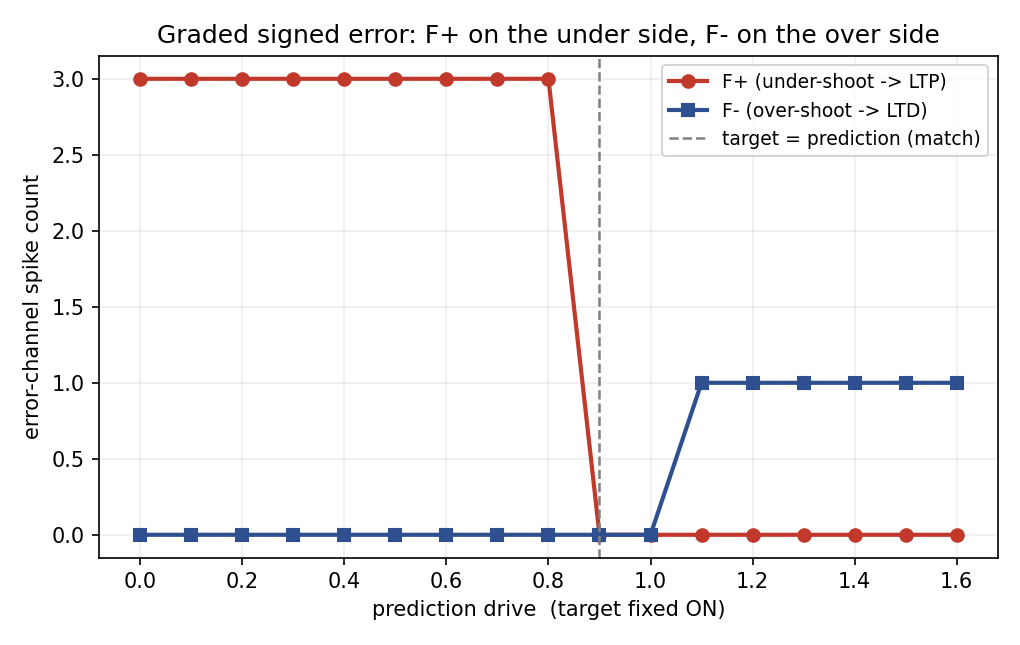
\includegraphics[width=0.78\textwidth]{exp3_graded_error.png}
\caption{Graded signed error. With the target fixed, $F^+$ (potentiation
driver) is active when the prediction under-shoots the target and $F^-$
(depression driver) is active when it over-shoots, with a near-silent
cross-over at match. The motif reads out the sign of the prediction error
without any global computation.}
\label{fig:spiking_graded}
\end{figure}

\subsection{Scope and limitations of the spiking validation}
\label{sec:spiking_scope}

\begin{remark}
This is a functional validation of the \emph{isolated} eight-neuron motif, not
of V1. It uses one neuron per role, current-based LIF dynamics with cell-type
membrane time constants, and hand-set synaptic weights; it does not include
plasticity (STDP), dendritic nonlinearities, conductance-based synapses,
short-term depression, or the recurrent embedding of the motif in the full
V1 graph. It therefore establishes that the signed-XOR computation is
\emph{realisable} in spiking dynamics with biologically plausible time
constants, and that this realisability is contingent on fast-spiking
inhibition --- but it does not establish that any particular V1 instance is
actually used this way \emph{in vivo}. Embedding the validated motif in the
Allen V1 reservoir, with cell-type-specific rates and STDP, is the natural
next step and is listed below.
\end{remark}

% --- New item for the validation plan in Section~\ref{sec:experiments} ---
% Insert the following \item into the enumerate in
% "Proposed experimental validation plan", e.g. as a new item 11.
%
% \item \textbf{Spiking functional validation (DONE, this paper,
%   \S\ref{sec:spiking}):} The isolated eight-neuron motif was simulated as a
%   cell-type-parameterised LIF network in Brian2. It reproduces the signed-XOR
%   truth table deterministically ($88\%$ under Poisson noise), produces a
%   correctly-signed graded error, and is functional \emph{only} with a
%   fast-spiking PV-type pivot ($\tau_m \leq 7$~ms; $0\%$ success at Sst/pyramidal
%   time constants), yielding the falsifiable Prediction~\ref{pred:pv}. Embedding
%   the validated motif in the full V1 reservoir with STDP remains follow-up work.

% --- Bibliography entry for Brian2 (paste into thebibliography, alpha order) ---
%
% \bibitem[Stimberg et~al., 2019]{Stimberg2019}
% Stimberg, M., Brette, R., and Goodman, D.~F.~M. (2019).
% \newblock Brian 2, an intuitive and efficient neural simulator.
% \newblock \emph{eLife}, 8:e47314.
%
% --- Optional addition to the Code and data availability section ---
%
% The spiking functional validation (Brian2/Python, \S\ref{sec:spiking}) is
% released as a standalone, MIT-licensed repository at
% \url{https://github.com/OWNER/signed-xor-motif-validation}; all figures and
% tables in this section are reproduced by a single \texttt{run\_all.py} script.
  after Section~\ref{sec:functional}
%      (the autoencoder reservoir experiment) and before the synthesis
%      Section~\ref{sec:synthesis}, OR keep it as its own top-level section
%      just before "Proposed experimental validation plan".
%   3. The block reuses the paper's existing environments
%      (prediction, conjecture, remark) and citation keys
%      (Billeh2020, Cardin2009, Atallah2012) -- no new packages needed.
%   4. Replace OWNER/REPO in the \url below with the public repository.
%
%  All numbers below are the actual output of the released code
%  (commit-pinned in results/*.json). Re-running run_all.py reproduces them.
% =====================================================================

\section{Functional validation: a spiking signed-XOR motif}
\label{sec:spiking}

The structural analysis (Sections~\ref{sec:scope}--\ref{sec:synthesis}) and
the reservoir experiment (Section~\ref{sec:functional}) treat the Allen V1
model as a static, signed graph; as stated in the Scope, they do not model
firing rates or spike timing, and a full functional characterisation
``requires spiking simulation with realistic rates.'' This section supplies
the minimal such characterisation for the \emph{isolated} eight-neuron motif.
The aim is narrow and deliberate: not to simulate V1, but to test whether the
signed-XOR computation defined in Section~\ref{sec:motif} actually emerges
from leaky integrate-and-fire (LIF) dynamics with mouse-V1 cell-type time
constants, and to convert the firing-rate caveat raised in the Abstract and in
Section~\ref{sec:scope} into a concrete, falsifiable prediction.

\subsection{Model}
\label{sec:spiking_model}

We instantiate the eight roles of Section~\ref{sec:motif}
($E_1, E_3$ inputs; $E_2, E_4$ latents; $\mathrm{INH}$ pivot;
$\mathrm{XOR}$ comparator; $F^+, F^-$ signed-error outputs) as current-based
LIF neurons in Brian2 \citep{Stimberg2019}, one neuron per role, wired with
the twelve directed edges of the motif. Membrane time constants are assigned
per Allen V1 cell type: thalamo-recipient inputs as \texttt{e4other}
($\tau_m=12$~ms), latents and comparator as \texttt{e23Cux2}
($\tau_m=15$~ms), and the inhibitory pivot as a fast-spiking
\texttt{i4Pvalb} interneuron ($\tau_m=6$~ms), reflecting the empirically
established $2$--$3\times$ faster membrane dynamics of parvalbumin cells
\citep{Cardin2009,Atallah2012}. The pivot implements the dual role argued for
in Section~\ref{sec:sparse_op}: it is wired as a \emph{coincidence detector},
firing only when both inputs are simultaneously active, and its veto of the
two latents is what realises the exclusive-or. The $F^+$ and $F^-$ neurons are
in turn coincidence detectors on (latent, comparator) pairs, so that they read
out the \emph{sign} of the mismatch. Each trial drives the active input(s) for
$100$~ms; a role is scored ``active'' if it emits $\geq 2$ spikes. Full
parameters, the synaptic weight matrix, and the integration scheme are in the
released code (Section~\ref{sec:availability}); the simulation uses Brian2's
pure-NumPy code-generation target and runs in seconds on a laptop under WSL.

\subsection{Result 1: the motif computes the signed-XOR truth table}
\label{sec:spiking_truth}

Driving the two inputs through all four binary conditions reproduces the
signed-XOR truth table of Section~\ref{sec:motif} deterministically
(Table~\ref{tab:spiking_truth}, Figure~\ref{fig:spiking_rasters}).
When the two inputs agree ($S_1=S_2$) the circuit rests in homeostasis with no
error signal: the silent case $(0,0)$ produces no spikes anywhere, and the
matched-active case $(1,1)$ drives the pivot ($8$ spikes) which vetoes both
latents, so the comparator and both error neurons stay silent. When the inputs
disagree, the comparator fires ($4$ spikes in both mismatch cases) and exactly
one error channel responds: the under-shoot case $(1,0)$ activates $F^+$
($3$ spikes, $F^-$ silent), the appropriate driver of potentiation, while the
over-shoot case $(0,1)$ activates $F^-$ ($7$ spikes, $F^+$ silent), the driver
of depression. The signed-error logic
$F^+ = \max(0, x-r)$, $F^- = \max(0, r-x)$ of Section~\ref{sec:dynamic} thus
holds at the level of spikes, not only in the rate abstraction.

\begin{table}[H]
\centering
\small
\begin{tabular}{cc cccccccc c}
\toprule
$S_1$ & $S_2$ & $E_1$ & $E_3$ & $E_2$ & $E_4$ & INH & XOR & $F^+$ & $F^-$ & interpretation \\
\midrule
0 & 0 & 0 & 0 & 0 & 0 & 0 & 0 & 0 & 0 & homeostasis (no error) \\
1 & 0 & 5 & 0 & 5 & 0 & 0 & 4 & 3 & 0 & under-shoot $\rightarrow$ LTP ($F^+$) \\
0 & 1 & 0 & 5 & 0 & 5 & 0 & 4 & 0 & 7 & over-shoot $\rightarrow$ LTD ($F^-$) \\
1 & 1 & 5 & 5 & 0 & 0 & 8 & 0 & 0 & 0 & homeostasis (matched) \\
\bottomrule
\end{tabular}
\caption{Spike counts per role over a $100$~ms trial for each input
condition. Entries are exact spike counts; a role is read out as active at
$\geq 2$ spikes. The comparator (XOR) is active iff the inputs differ, and the
two error channels $F^+/F^-$ partition the two mismatch directions. The table
is reproduced deterministically; under $20$~Hz Poisson background noise (25
random seeds) the full four-row table is recovered on $88\%$ of trials.}
\label{tab:spiking_truth}
\end{table}

\begin{figure}[H]
\centering
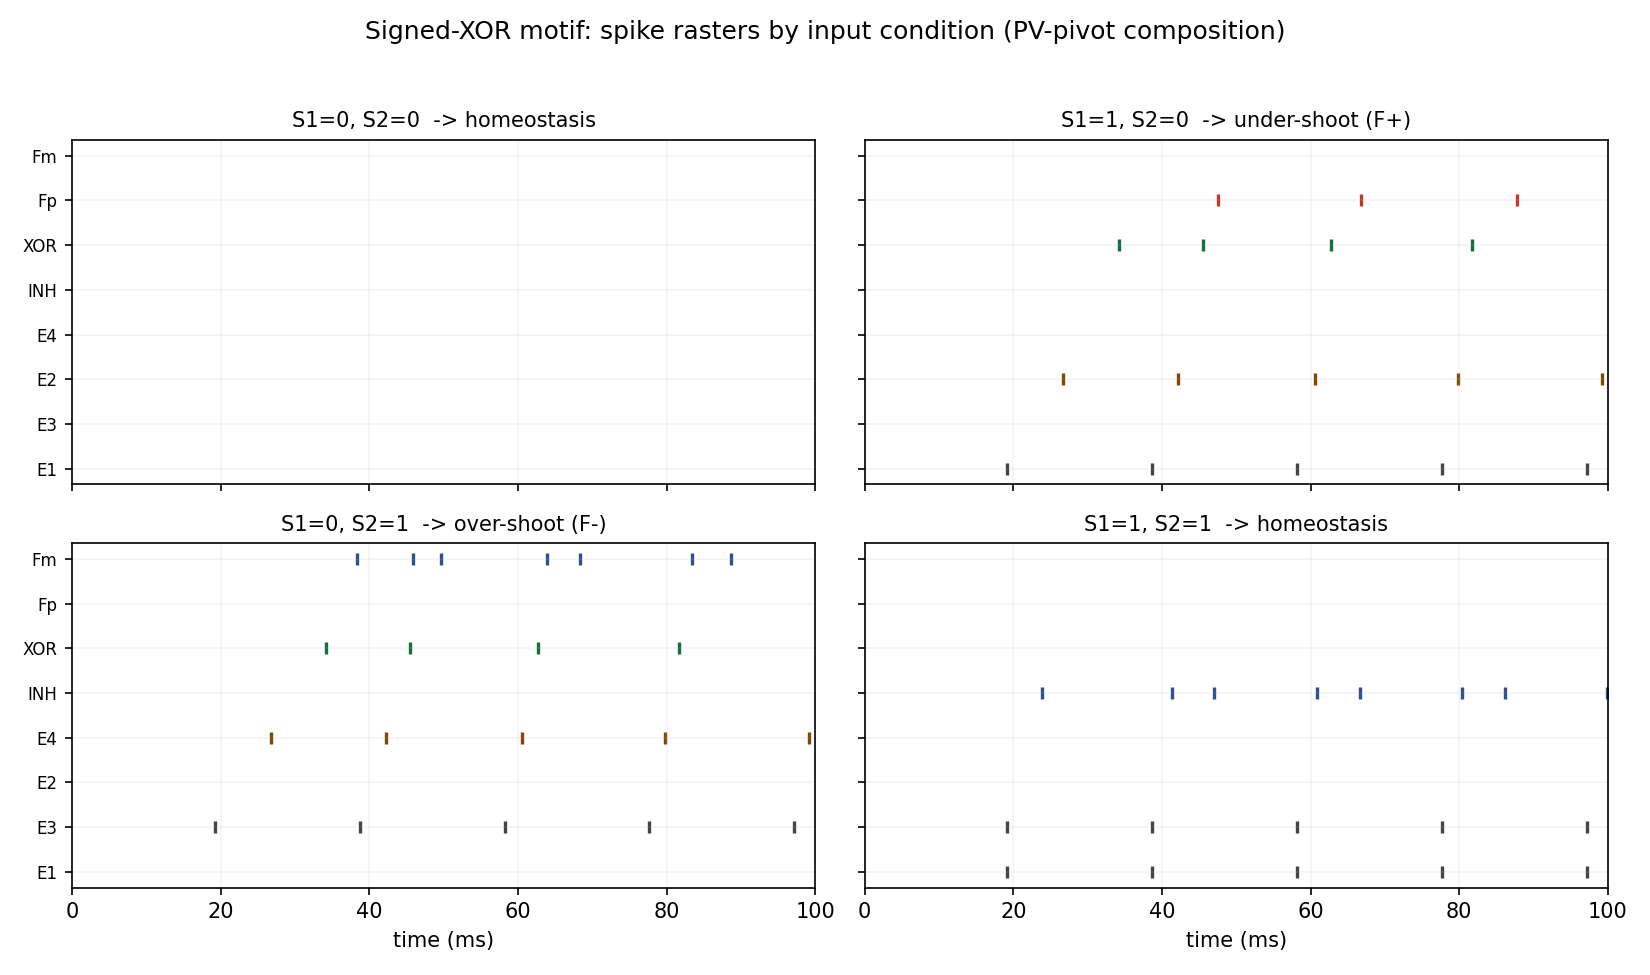
\includegraphics[width=\textwidth]{exp1_rasters.png}
\caption{Spike rasters of the eight motif neurons for the four input
conditions. The inhibitory pivot (INH) fires only when both inputs are
co-active $(1,1)$ and silences the latents; the comparator (XOR) fires only on
mismatch; $F^+$ and $F^-$ each respond to exactly one mismatch direction.}
\label{fig:spiking_rasters}
\end{figure}

\subsection{Result 2: fast-spiking inhibition is required}
\label{sec:spiking_pv}

The coincidence/veto logic of the pivot depends on its membrane integration
window being short relative to the synaptic time scale: a slow pivot integrates
a single input up to threshold and fires spuriously, destroying the exclusive-
or. We tested this directly by sweeping the pivot's membrane time constant
$\tau_m^{\mathrm{INH}}$ from $4$ to $15$~ms while holding everything else fixed,
scoring the full truth table over 15 noisy seeds per value
(Figure~\ref{fig:spiking_pv}). The circuit succeeds on $100\%$ of trials for
$\tau_m^{\mathrm{INH}} \in [6,7]$~ms (fast-spiking, PV-like), degrades through
$\tau_m^{\mathrm{INH}}=8$~ms ($60\%$), and fails completely
($0\%$) for $\tau_m^{\mathrm{INH}} \geq 9$~ms --- i.e.\ at the membrane time
constants of pyramidal ($\sim12$--$15$~ms) or somatostatin/Htr3a interneurons
($\sim10$--$12$~ms). Consistently, instantiating the pivot with the
\texttt{i4Pvalb} cell type yields a working circuit, whereas instantiating it
with the rank-1 empirical \texttt{i4Sst} pivot reported in
Section~\ref{sec:weight_stats} does \emph{not}, at otherwise identical
parameters.

\begin{figure}[H]
\centering
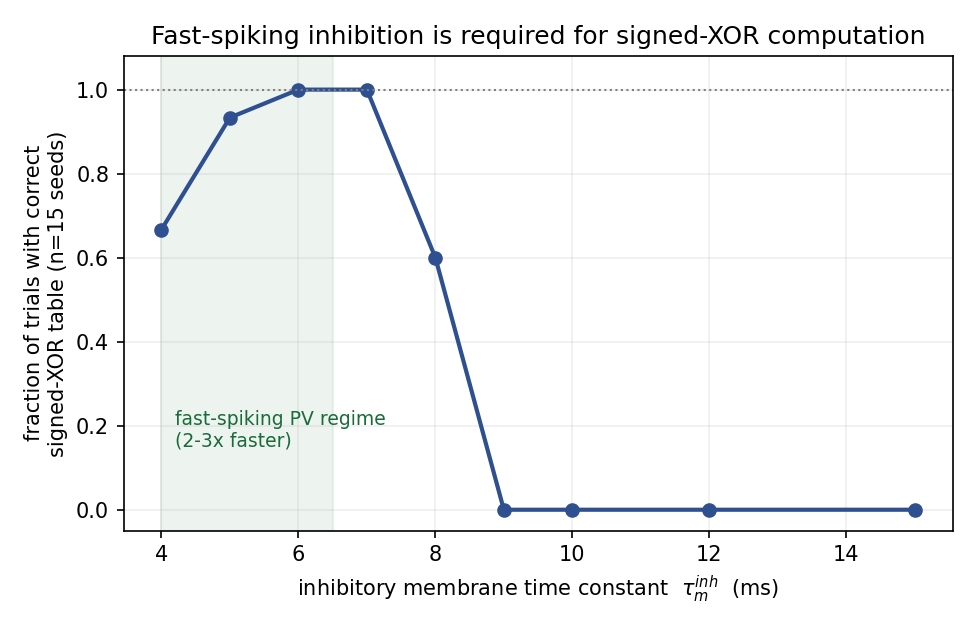
\includegraphics[width=0.78\textwidth]{exp2_pv_sweep.png}
\caption{Truth-table success rate (15 noisy seeds per point) as a function of
the inhibitory pivot's membrane time constant. The functional window
($100\%$ success) is confined to the fast-spiking, parvalbumin-like regime
($\tau_m \leq 7$~ms); the computation collapses at pyramidal and
Sst/Htr3a-like time constants.}
\label{fig:spiking_pv}
\end{figure}

This turns the firing-rate caveat of the Abstract and Section~\ref{sec:scope}
into a sharp, testable claim. The structural analysis is cell-type-agnostic
about which inhibitory subtype occupies the pivot; the dynamics are not.

\begin{prediction}{Fast-spiking pivot requirement}{pv}
A signed-XOR motif instance is \emph{functional} (computes the exclusive-or and
its signed error) only if its inhibitory pivot is a fast-spiking,
parvalbumin-type interneuron. Motif instances whose pivot is a somatostatin- or
Htr3a/VIP-type interneuron are structurally present but functionally inert
under realistic membrane time constants. Equivalently: the functional density
of the motif in cortex is bounded above by the density of \emph{PV-pivoted}
instances, which can be substantially lower than the structural density counted
on the static graph.
\end{prediction}

This prediction is directly falsifiable, both \emph{in silico} (a full
cell-type-resolved spiking simulation of the Allen V1 model should find error-
correlated activity concentrated on PV-pivoted instances) and \emph{in vivo}
(optogenetic silencing of PV vs.\ Sst interneurons should differentially
abolish mismatch responses in candidate motif circuits). It also refines the
structural counts of Section~\ref{sec:weight_stats}: the i4Pvalb dominance
observed at the stricter weight threshold $|w|\geq 1.0$ is, on this account,
the functionally relevant population, while the Sst-pivoted instances dominant
at $|w|\geq 0.1$ may be structural background.

\subsection{Result 3: the error signal is graded and correctly signed}
\label{sec:spiking_graded}

Finally we tested the graded regime of Section~\ref{sec:dynamic}. Holding the
``target'' input fixed and sweeping the ``prediction'' input from $0$ to
$1.6\times$ its level, $F^+$ fires at a fixed rate on the entire under-shoot
side (prediction below target) and falls silent once the prediction reaches the
target, while $F^-$ is silent on the under-shoot side and activates on the
over-shoot side (Figure~\ref{fig:spiking_graded}). The cross-over (minimum
error, both channels near silent) occurs at $\approx 0.9\times$ the target,
i.e.\ near match, recovering the homeostatic stopping condition. The two
channels therefore encode the sign of the mismatch with the correct polarity,
as required by the energy decomposition of Section~\ref{sec:energy}.

\begin{figure}[H]
\centering
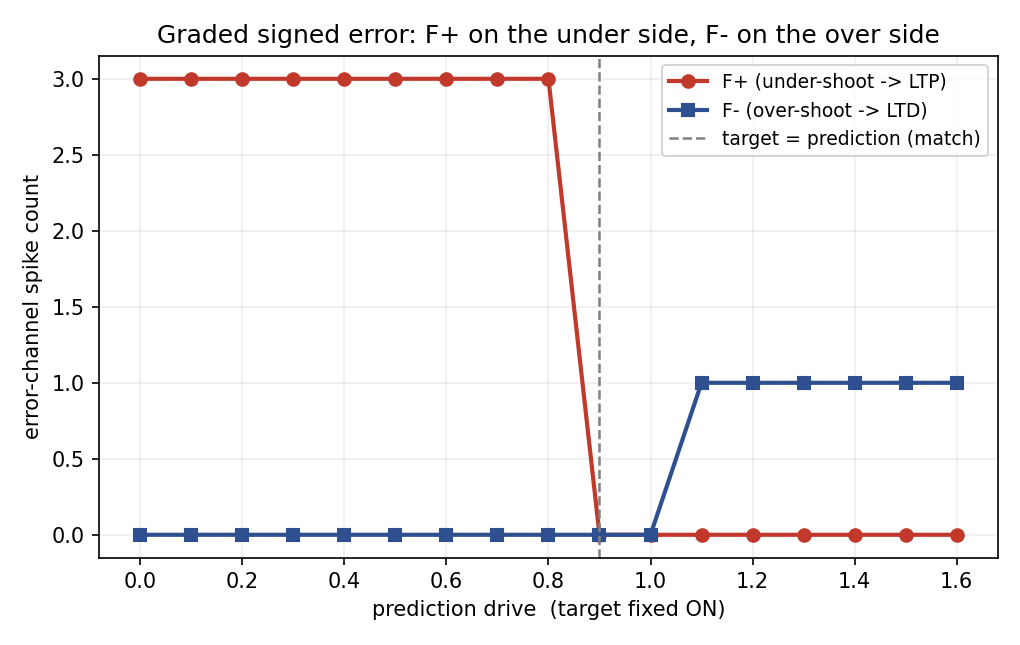
\includegraphics[width=0.78\textwidth]{exp3_graded_error.png}
\caption{Graded signed error. With the target fixed, $F^+$ (potentiation
driver) is active when the prediction under-shoots the target and $F^-$
(depression driver) is active when it over-shoots, with a near-silent
cross-over at match. The motif reads out the sign of the prediction error
without any global computation.}
\label{fig:spiking_graded}
\end{figure}

\subsection{Scope and limitations of the spiking validation}
\label{sec:spiking_scope}

\begin{remark}
This is a functional validation of the \emph{isolated} eight-neuron motif, not
of V1. It uses one neuron per role, current-based LIF dynamics with cell-type
membrane time constants, and hand-set synaptic weights; it does not include
plasticity (STDP), dendritic nonlinearities, conductance-based synapses,
short-term depression, or the recurrent embedding of the motif in the full
V1 graph. It therefore establishes that the signed-XOR computation is
\emph{realisable} in spiking dynamics with biologically plausible time
constants, and that this realisability is contingent on fast-spiking
inhibition --- but it does not establish that any particular V1 instance is
actually used this way \emph{in vivo}. Embedding the validated motif in the
Allen V1 reservoir, with cell-type-specific rates and STDP, is the natural
next step and is listed below.
\end{remark}

% --- New item for the validation plan in Section~\ref{sec:experiments} ---
% Insert the following \item into the enumerate in
% "Proposed experimental validation plan", e.g. as a new item 11.
%
% \item \textbf{Spiking functional validation (DONE, this paper,
%   \S\ref{sec:spiking}):} The isolated eight-neuron motif was simulated as a
%   cell-type-parameterised LIF network in Brian2. It reproduces the signed-XOR
%   truth table deterministically ($88\%$ under Poisson noise), produces a
%   correctly-signed graded error, and is functional \emph{only} with a
%   fast-spiking PV-type pivot ($\tau_m \leq 7$~ms; $0\%$ success at Sst/pyramidal
%   time constants), yielding the falsifiable Prediction~\ref{pred:pv}. Embedding
%   the validated motif in the full V1 reservoir with STDP remains follow-up work.

% --- Bibliography entry for Brian2 (paste into thebibliography, alpha order) ---
%
% \bibitem[Stimberg et~al., 2019]{Stimberg2019}
% Stimberg, M., Brette, R., and Goodman, D.~F.~M. (2019).
% \newblock Brian 2, an intuitive and efficient neural simulator.
% \newblock \emph{eLife}, 8:e47314.
%
% --- Optional addition to the Code and data availability section ---
%
% The spiking functional validation (Brian2/Python, \S\ref{sec:spiking}) is
% released as a standalone, MIT-licensed repository at
% \url{https://github.com/OWNER/signed-xor-motif-validation}; all figures and
% tables in this section are reproduced by a single \texttt{run\_all.py} script.
  after Section~\ref{sec:functional}
%      (the autoencoder reservoir experiment) and before the synthesis
%      Section~\ref{sec:synthesis}, OR keep it as its own top-level section
%      just before "Proposed experimental validation plan".
%   3. The block reuses the paper's existing environments
%      (prediction, conjecture, remark) and citation keys
%      (Billeh2020, Cardin2009, Atallah2012) -- no new packages needed.
%   4. Replace OWNER/REPO in the \url below with the public repository.
%
%  All numbers below are the actual output of the released code
%  (commit-pinned in results/*.json). Re-running run_all.py reproduces them.
% =====================================================================

\section{Functional validation: a spiking signed-XOR motif}
\label{sec:spiking}

The structural analysis (Sections~\ref{sec:scope}--\ref{sec:synthesis}) and
the reservoir experiment (Section~\ref{sec:functional}) treat the Allen V1
model as a static, signed graph; as stated in the Scope, they do not model
firing rates or spike timing, and a full functional characterisation
``requires spiking simulation with realistic rates.'' This section supplies
the minimal such characterisation for the \emph{isolated} eight-neuron motif.
The aim is narrow and deliberate: not to simulate V1, but to test whether the
signed-XOR computation defined in Section~\ref{sec:motif} actually emerges
from leaky integrate-and-fire (LIF) dynamics with mouse-V1 cell-type time
constants, and to convert the firing-rate caveat raised in the Abstract and in
Section~\ref{sec:scope} into a concrete, falsifiable prediction.

\subsection{Model}
\label{sec:spiking_model}

We instantiate the eight roles of Section~\ref{sec:motif}
($E_1, E_3$ inputs; $E_2, E_4$ latents; $\mathrm{INH}$ pivot;
$\mathrm{XOR}$ comparator; $F^+, F^-$ signed-error outputs) as current-based
LIF neurons in Brian2 \citep{Stimberg2019}, one neuron per role, wired with
the twelve directed edges of the motif. Membrane time constants are assigned
per Allen V1 cell type: thalamo-recipient inputs as \texttt{e4other}
($\tau_m=12$~ms), latents and comparator as \texttt{e23Cux2}
($\tau_m=15$~ms), and the inhibitory pivot as a fast-spiking
\texttt{i4Pvalb} interneuron ($\tau_m=6$~ms), reflecting the empirically
established $2$--$3\times$ faster membrane dynamics of parvalbumin cells
\citep{Cardin2009,Atallah2012}. The pivot implements the dual role argued for
in Section~\ref{sec:sparse_op}: it is wired as a \emph{coincidence detector},
firing only when both inputs are simultaneously active, and its veto of the
two latents is what realises the exclusive-or. The $F^+$ and $F^-$ neurons are
in turn coincidence detectors on (latent, comparator) pairs, so that they read
out the \emph{sign} of the mismatch. Each trial drives the active input(s) for
$100$~ms; a role is scored ``active'' if it emits $\geq 2$ spikes. Full
parameters, the synaptic weight matrix, and the integration scheme are in the
released code (Section~\ref{sec:availability}); the simulation uses Brian2's
pure-NumPy code-generation target and runs in seconds on a laptop under WSL.

\subsection{Result 1: the motif computes the signed-XOR truth table}
\label{sec:spiking_truth}

Driving the two inputs through all four binary conditions reproduces the
signed-XOR truth table of Section~\ref{sec:motif} deterministically
(Table~\ref{tab:spiking_truth}, Figure~\ref{fig:spiking_rasters}).
When the two inputs agree ($S_1=S_2$) the circuit rests in homeostasis with no
error signal: the silent case $(0,0)$ produces no spikes anywhere, and the
matched-active case $(1,1)$ drives the pivot ($8$ spikes) which vetoes both
latents, so the comparator and both error neurons stay silent. When the inputs
disagree, the comparator fires ($4$ spikes in both mismatch cases) and exactly
one error channel responds: the under-shoot case $(1,0)$ activates $F^+$
($3$ spikes, $F^-$ silent), the appropriate driver of potentiation, while the
over-shoot case $(0,1)$ activates $F^-$ ($7$ spikes, $F^+$ silent), the driver
of depression. The signed-error logic
$F^+ = \max(0, x-r)$, $F^- = \max(0, r-x)$ of Section~\ref{sec:dynamic} thus
holds at the level of spikes, not only in the rate abstraction.

\begin{table}[H]
\centering
\small
\begin{tabular}{cc cccccccc c}
\toprule
$S_1$ & $S_2$ & $E_1$ & $E_3$ & $E_2$ & $E_4$ & INH & XOR & $F^+$ & $F^-$ & interpretation \\
\midrule
0 & 0 & 0 & 0 & 0 & 0 & 0 & 0 & 0 & 0 & homeostasis (no error) \\
1 & 0 & 5 & 0 & 5 & 0 & 0 & 4 & 3 & 0 & under-shoot $\rightarrow$ LTP ($F^+$) \\
0 & 1 & 0 & 5 & 0 & 5 & 0 & 4 & 0 & 7 & over-shoot $\rightarrow$ LTD ($F^-$) \\
1 & 1 & 5 & 5 & 0 & 0 & 8 & 0 & 0 & 0 & homeostasis (matched) \\
\bottomrule
\end{tabular}
\caption{Spike counts per role over a $100$~ms trial for each input
condition. Entries are exact spike counts; a role is read out as active at
$\geq 2$ spikes. The comparator (XOR) is active iff the inputs differ, and the
two error channels $F^+/F^-$ partition the two mismatch directions. The table
is reproduced deterministically; under $20$~Hz Poisson background noise (25
random seeds) the full four-row table is recovered on $88\%$ of trials.}
\label{tab:spiking_truth}
\end{table}

\begin{figure}[H]
\centering
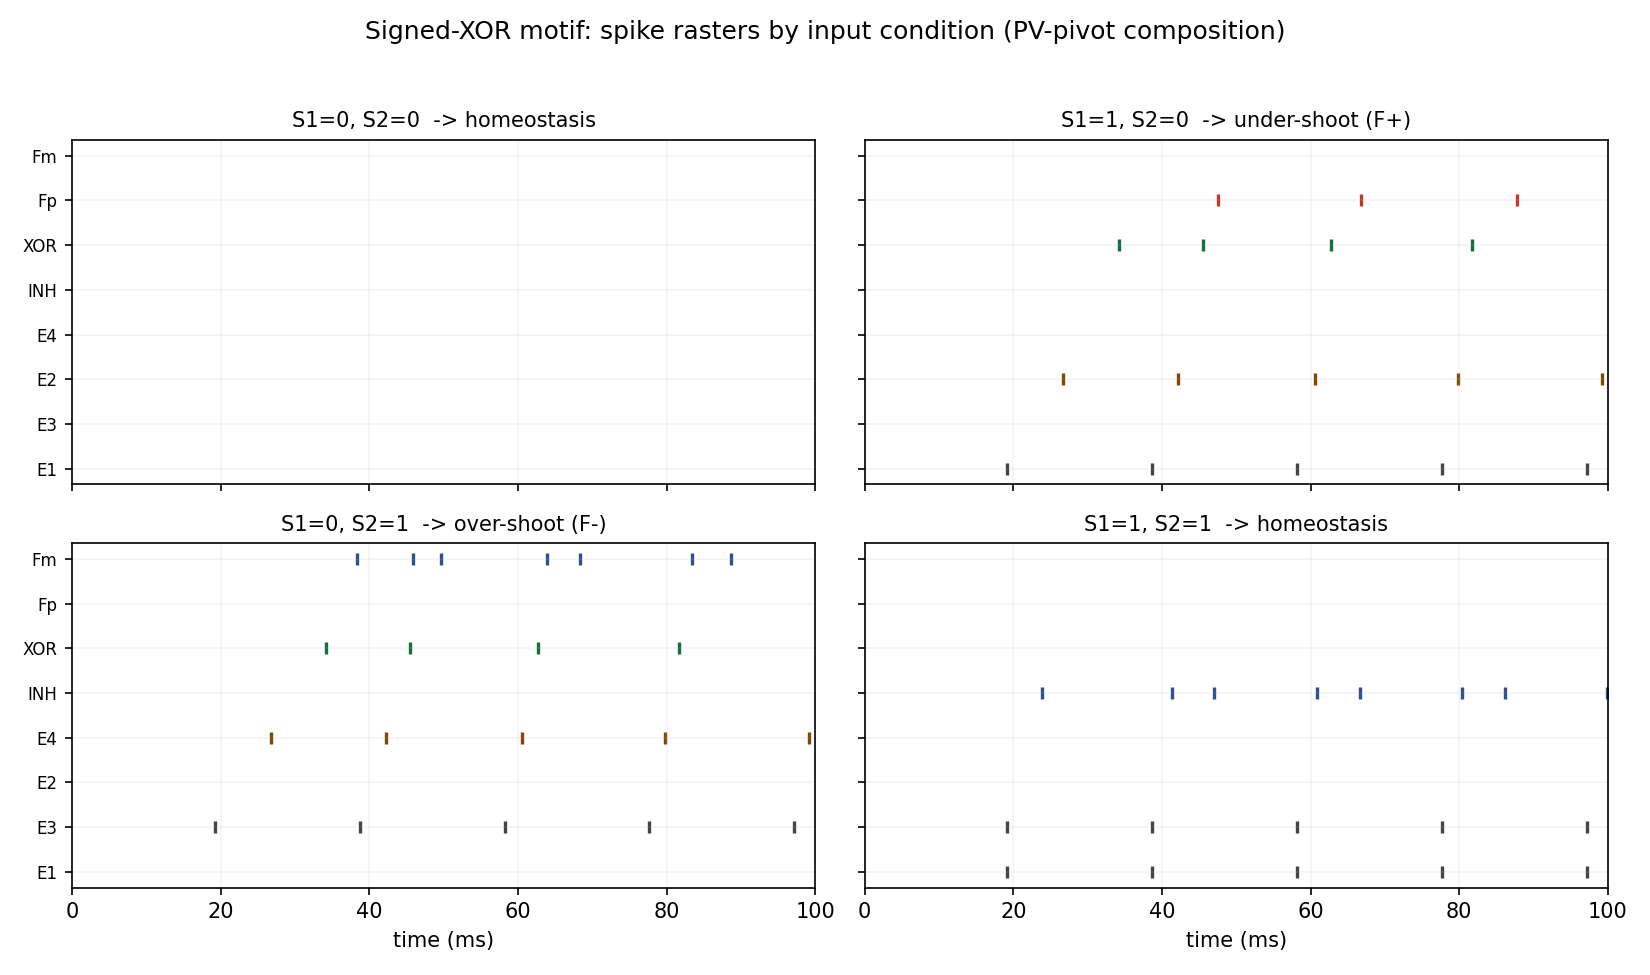
\includegraphics[width=\textwidth]{exp1_rasters.png}
\caption{Spike rasters of the eight motif neurons for the four input
conditions. The inhibitory pivot (INH) fires only when both inputs are
co-active $(1,1)$ and silences the latents; the comparator (XOR) fires only on
mismatch; $F^+$ and $F^-$ each respond to exactly one mismatch direction.}
\label{fig:spiking_rasters}
\end{figure}

\subsection{Result 2: fast-spiking inhibition is required}
\label{sec:spiking_pv}

The coincidence/veto logic of the pivot depends on its membrane integration
window being short relative to the synaptic time scale: a slow pivot integrates
a single input up to threshold and fires spuriously, destroying the exclusive-
or. We tested this directly by sweeping the pivot's membrane time constant
$\tau_m^{\mathrm{INH}}$ from $4$ to $15$~ms while holding everything else fixed,
scoring the full truth table over 15 noisy seeds per value
(Figure~\ref{fig:spiking_pv}). The circuit succeeds on $100\%$ of trials for
$\tau_m^{\mathrm{INH}} \in [6,7]$~ms (fast-spiking, PV-like), degrades through
$\tau_m^{\mathrm{INH}}=8$~ms ($60\%$), and fails completely
($0\%$) for $\tau_m^{\mathrm{INH}} \geq 9$~ms --- i.e.\ at the membrane time
constants of pyramidal ($\sim12$--$15$~ms) or somatostatin/Htr3a interneurons
($\sim10$--$12$~ms). Consistently, instantiating the pivot with the
\texttt{i4Pvalb} cell type yields a working circuit, whereas instantiating it
with the rank-1 empirical \texttt{i4Sst} pivot reported in
Section~\ref{sec:weight_stats} does \emph{not}, at otherwise identical
parameters.

\begin{figure}[H]
\centering
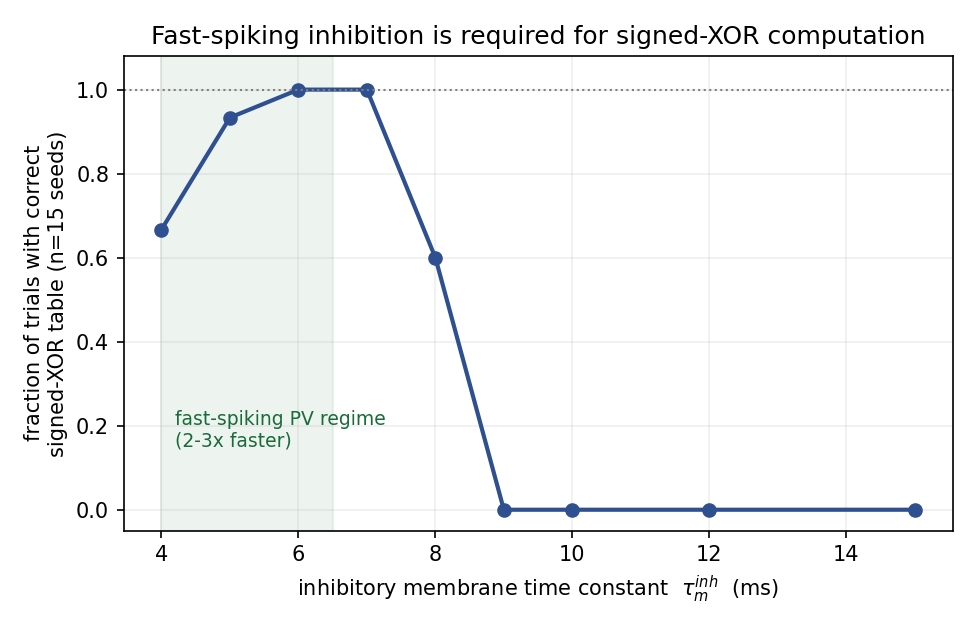
\includegraphics[width=0.78\textwidth]{exp2_pv_sweep.png}
\caption{Truth-table success rate (15 noisy seeds per point) as a function of
the inhibitory pivot's membrane time constant. The functional window
($100\%$ success) is confined to the fast-spiking, parvalbumin-like regime
($\tau_m \leq 7$~ms); the computation collapses at pyramidal and
Sst/Htr3a-like time constants.}
\label{fig:spiking_pv}
\end{figure}

This turns the firing-rate caveat of the Abstract and Section~\ref{sec:scope}
into a sharp, testable claim. The structural analysis is cell-type-agnostic
about which inhibitory subtype occupies the pivot; the dynamics are not.

\begin{prediction}{Fast-spiking pivot requirement}{pv}
A signed-XOR motif instance is \emph{functional} (computes the exclusive-or and
its signed error) only if its inhibitory pivot is a fast-spiking,
parvalbumin-type interneuron. Motif instances whose pivot is a somatostatin- or
Htr3a/VIP-type interneuron are structurally present but functionally inert
under realistic membrane time constants. Equivalently: the functional density
of the motif in cortex is bounded above by the density of \emph{PV-pivoted}
instances, which can be substantially lower than the structural density counted
on the static graph.
\end{prediction}

This prediction is directly falsifiable, both \emph{in silico} (a full
cell-type-resolved spiking simulation of the Allen V1 model should find error-
correlated activity concentrated on PV-pivoted instances) and \emph{in vivo}
(optogenetic silencing of PV vs.\ Sst interneurons should differentially
abolish mismatch responses in candidate motif circuits). It also refines the
structural counts of Section~\ref{sec:weight_stats}: the i4Pvalb dominance
observed at the stricter weight threshold $|w|\geq 1.0$ is, on this account,
the functionally relevant population, while the Sst-pivoted instances dominant
at $|w|\geq 0.1$ may be structural background.

\subsection{Result 3: the error signal is graded and correctly signed}
\label{sec:spiking_graded}

Finally we tested the graded regime of Section~\ref{sec:dynamic}. Holding the
``target'' input fixed and sweeping the ``prediction'' input from $0$ to
$1.6\times$ its level, $F^+$ fires at a fixed rate on the entire under-shoot
side (prediction below target) and falls silent once the prediction reaches the
target, while $F^-$ is silent on the under-shoot side and activates on the
over-shoot side (Figure~\ref{fig:spiking_graded}). The cross-over (minimum
error, both channels near silent) occurs at $\approx 0.9\times$ the target,
i.e.\ near match, recovering the homeostatic stopping condition. The two
channels therefore encode the sign of the mismatch with the correct polarity,
as required by the energy decomposition of Section~\ref{sec:energy}.

\begin{figure}[H]
\centering
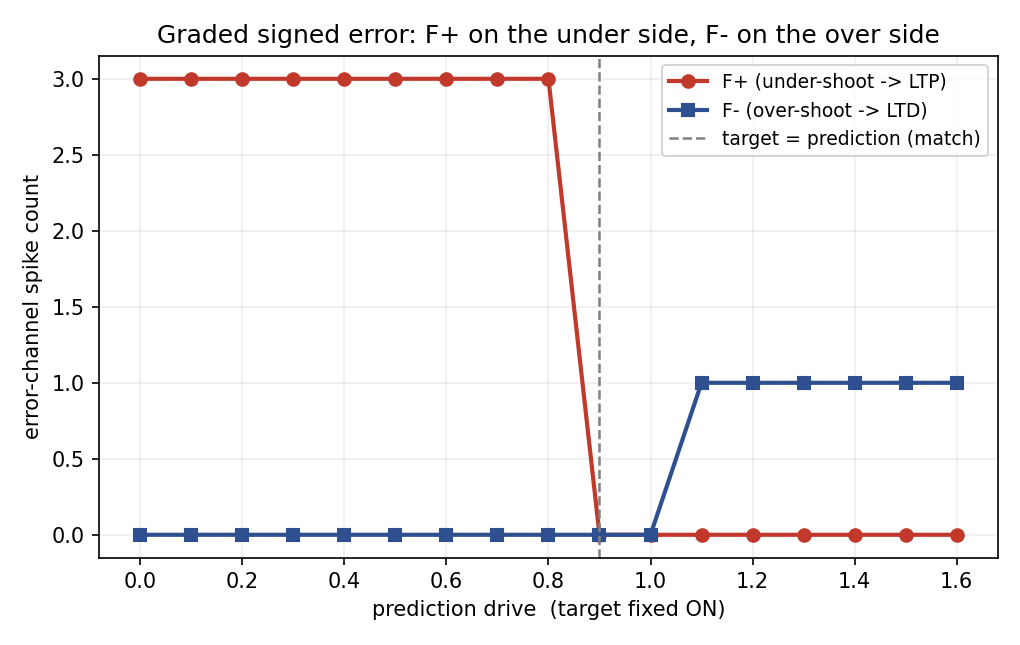
\includegraphics[width=0.78\textwidth]{exp3_graded_error.png}
\caption{Graded signed error. With the target fixed, $F^+$ (potentiation
driver) is active when the prediction under-shoots the target and $F^-$
(depression driver) is active when it over-shoots, with a near-silent
cross-over at match. The motif reads out the sign of the prediction error
without any global computation.}
\label{fig:spiking_graded}
\end{figure}

\subsection{Scope and limitations of the spiking validation}
\label{sec:spiking_scope}

\begin{remark}
This is a functional validation of the \emph{isolated} eight-neuron motif, not
of V1. It uses one neuron per role, current-based LIF dynamics with cell-type
membrane time constants, and hand-set synaptic weights; it does not include
plasticity (STDP), dendritic nonlinearities, conductance-based synapses,
short-term depression, or the recurrent embedding of the motif in the full
V1 graph. It therefore establishes that the signed-XOR computation is
\emph{realisable} in spiking dynamics with biologically plausible time
constants, and that this realisability is contingent on fast-spiking
inhibition --- but it does not establish that any particular V1 instance is
actually used this way \emph{in vivo}. Embedding the validated motif in the
Allen V1 reservoir, with cell-type-specific rates and STDP, is the natural
next step and is listed below.
\end{remark}

% --- New item for the validation plan in Section~\ref{sec:experiments} ---
% Insert the following \item into the enumerate in
% "Proposed experimental validation plan", e.g. as a new item 11.
%
% \item \textbf{Spiking functional validation (DONE, this paper,
%   \S\ref{sec:spiking}):} The isolated eight-neuron motif was simulated as a
%   cell-type-parameterised LIF network in Brian2. It reproduces the signed-XOR
%   truth table deterministically ($88\%$ under Poisson noise), produces a
%   correctly-signed graded error, and is functional \emph{only} with a
%   fast-spiking PV-type pivot ($\tau_m \leq 7$~ms; $0\%$ success at Sst/pyramidal
%   time constants), yielding the falsifiable Prediction~\ref{pred:pv}. Embedding
%   the validated motif in the full V1 reservoir with STDP remains follow-up work.

% --- Bibliography entry for Brian2 (paste into thebibliography, alpha order) ---
%
% \bibitem[Stimberg et~al., 2019]{Stimberg2019}
% Stimberg, M., Brette, R., and Goodman, D.~F.~M. (2019).
% \newblock Brian 2, an intuitive and efficient neural simulator.
% \newblock \emph{eLife}, 8:e47314.
%
% --- Optional addition to the Code and data availability section ---
%
% The spiking functional validation (Brian2/Python, \S\ref{sec:spiking}) is
% released as a standalone, MIT-licensed repository at
% \url{https://github.com/OWNER/signed-xor-motif-validation}; all figures and
% tables in this section are reproduced by a single \texttt{run\_all.py} script.
  after Section~\ref{sec:functional}
%      (the autoencoder reservoir experiment) and before the synthesis
%      Section~\ref{sec:synthesis}, OR keep it as its own top-level section
%      just before "Proposed experimental validation plan".
%   3. The block reuses the paper's existing environments
%      (prediction, conjecture, remark) and citation keys
%      (Billeh2020, Cardin2009, Atallah2012) -- no new packages needed.
%   4. Replace OWNER/REPO in the \url below with the public repository.
%
%  All numbers below are the actual output of the released code
%  (commit-pinned in results/*.json). Re-running run_all.py reproduces them.
% =====================================================================

\section{Functional validation: a spiking signed-XOR motif}
\label{sec:spiking}

The structural analysis (Sections~\ref{sec:scope}--\ref{sec:synthesis}) and
the reservoir experiment (Section~\ref{sec:functional}) treat the Allen V1
model as a static, signed graph; as stated in the Scope, they do not model
firing rates or spike timing, and a full functional characterisation
``requires spiking simulation with realistic rates.'' This section supplies
the minimal such characterisation for the \emph{isolated} eight-neuron motif.
The aim is narrow and deliberate: not to simulate V1, but to test whether the
signed-XOR computation defined in Section~\ref{sec:motif} actually emerges
from leaky integrate-and-fire (LIF) dynamics with mouse-V1 cell-type time
constants, and to convert the firing-rate caveat raised in the Abstract and in
Section~\ref{sec:scope} into a concrete, falsifiable prediction.

\subsection{Model}
\label{sec:spiking_model}

We instantiate the eight roles of Section~\ref{sec:motif}
($E_1, E_3$ inputs; $E_2, E_4$ latents; $\mathrm{INH}$ pivot;
$\mathrm{XOR}$ comparator; $F^+, F^-$ signed-error outputs) as current-based
LIF neurons in Brian2 \citep{Stimberg2019}, one neuron per role, wired with
the twelve directed edges of the motif. Membrane time constants are assigned
per Allen V1 cell type: thalamo-recipient inputs as \texttt{e4other}
($\tau_m=12$~ms), latents and comparator as \texttt{e23Cux2}
($\tau_m=15$~ms), and the inhibitory pivot as a fast-spiking
\texttt{i4Pvalb} interneuron ($\tau_m=6$~ms), reflecting the empirically
established $2$--$3\times$ faster membrane dynamics of parvalbumin cells
\citep{Cardin2009,Atallah2012}. The pivot implements the dual role argued for
in Section~\ref{sec:sparse_op}: it is wired as a \emph{coincidence detector},
firing only when both inputs are simultaneously active, and its veto of the
two latents is what realises the exclusive-or. The $F^+$ and $F^-$ neurons are
in turn coincidence detectors on (latent, comparator) pairs, so that they read
out the \emph{sign} of the mismatch. Each trial drives the active input(s) for
$100$~ms; a role is scored ``active'' if it emits $\geq 2$ spikes. Full
parameters, the synaptic weight matrix, and the integration scheme are in the
released code (Section~\ref{sec:availability}); the simulation uses Brian2's
pure-NumPy code-generation target and runs in seconds on a laptop under WSL.

\subsection{Result 1: the motif computes the signed-XOR truth table}
\label{sec:spiking_truth}

Driving the two inputs through all four binary conditions reproduces the
signed-XOR truth table of Section~\ref{sec:motif} deterministically
(Table~\ref{tab:spiking_truth}, Figure~\ref{fig:spiking_rasters}).
When the two inputs agree ($S_1=S_2$) the circuit rests in homeostasis with no
error signal: the silent case $(0,0)$ produces no spikes anywhere, and the
matched-active case $(1,1)$ drives the pivot ($8$ spikes) which vetoes both
latents, so the comparator and both error neurons stay silent. When the inputs
disagree, the comparator fires ($4$ spikes in both mismatch cases) and exactly
one error channel responds: the under-shoot case $(1,0)$ activates $F^+$
($3$ spikes, $F^-$ silent), the appropriate driver of potentiation, while the
over-shoot case $(0,1)$ activates $F^-$ ($7$ spikes, $F^+$ silent), the driver
of depression. The signed-error logic
$F^+ = \max(0, x-r)$, $F^- = \max(0, r-x)$ of Section~\ref{sec:dynamic} thus
holds at the level of spikes, not only in the rate abstraction.

\begin{table}[H]
\centering
\small
\begin{tabular}{cc cccccccc c}
\toprule
$S_1$ & $S_2$ & $E_1$ & $E_3$ & $E_2$ & $E_4$ & INH & XOR & $F^+$ & $F^-$ & interpretation \\
\midrule
0 & 0 & 0 & 0 & 0 & 0 & 0 & 0 & 0 & 0 & homeostasis (no error) \\
1 & 0 & 5 & 0 & 5 & 0 & 0 & 4 & 3 & 0 & under-shoot $\rightarrow$ LTP ($F^+$) \\
0 & 1 & 0 & 5 & 0 & 5 & 0 & 4 & 0 & 7 & over-shoot $\rightarrow$ LTD ($F^-$) \\
1 & 1 & 5 & 5 & 0 & 0 & 8 & 0 & 0 & 0 & homeostasis (matched) \\
\bottomrule
\end{tabular}
\caption{Spike counts per role over a $100$~ms trial for each input
condition. Entries are exact spike counts; a role is read out as active at
$\geq 2$ spikes. The comparator (XOR) is active iff the inputs differ, and the
two error channels $F^+/F^-$ partition the two mismatch directions. The table
is reproduced deterministically; under $20$~Hz Poisson background noise (25
random seeds) the full four-row table is recovered on $88\%$ of trials.}
\label{tab:spiking_truth}
\end{table}

\begin{figure}[H]
\centering
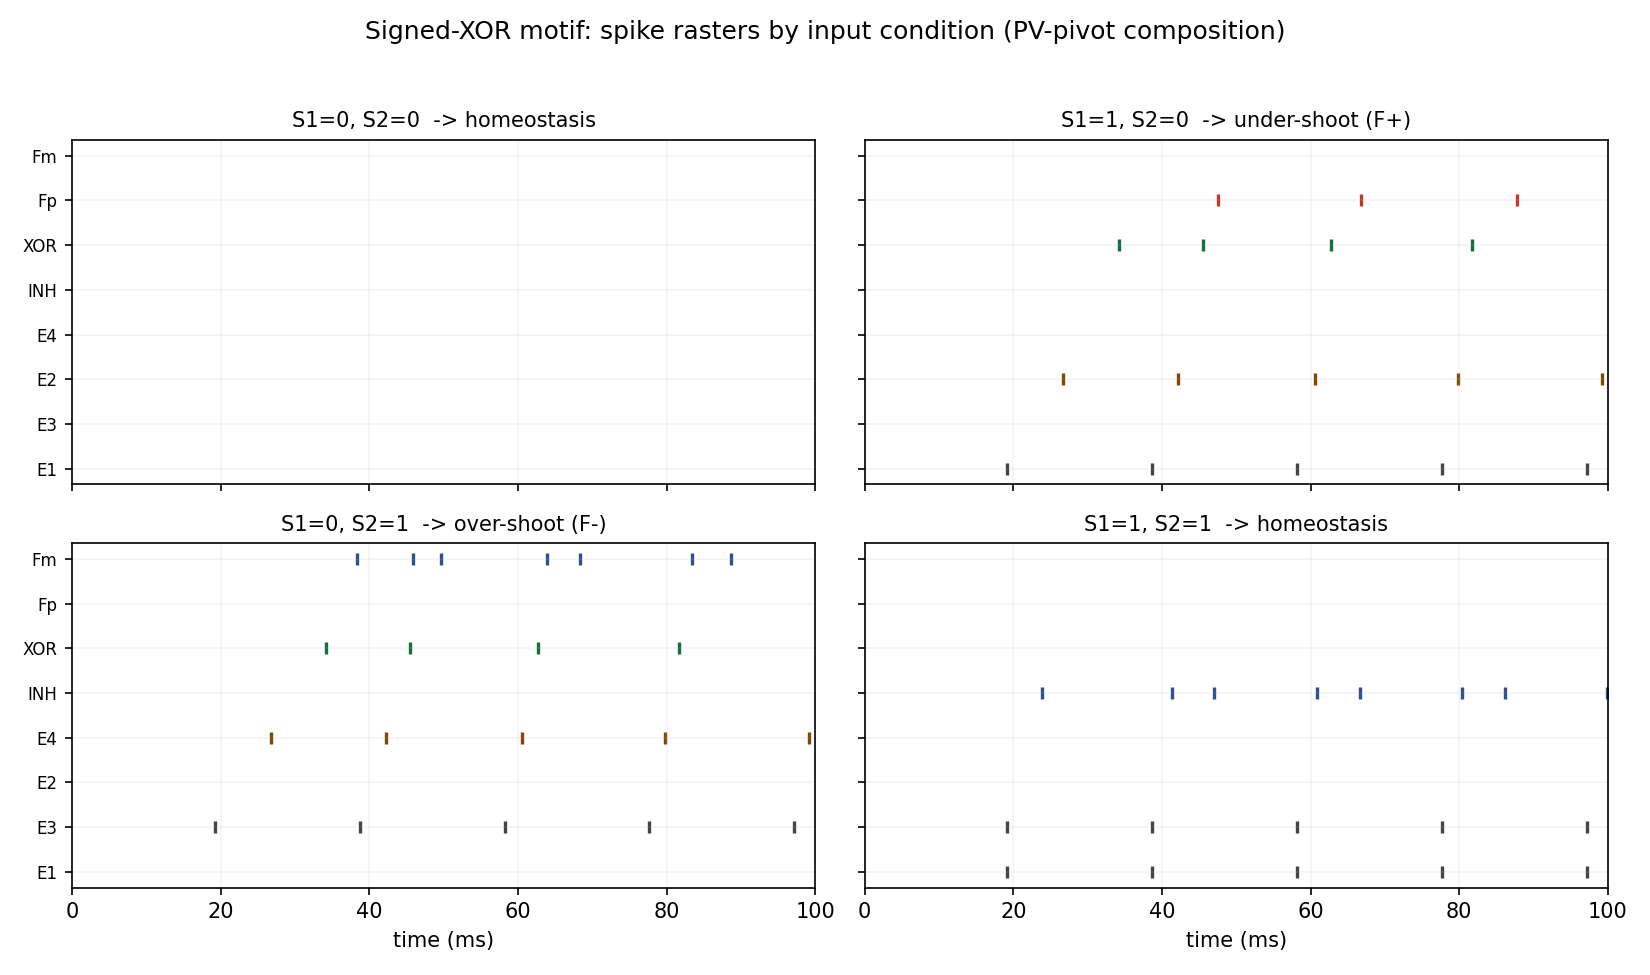
\includegraphics[width=\textwidth]{exp1_rasters.png}
\caption{Spike rasters of the eight motif neurons for the four input
conditions. The inhibitory pivot (INH) fires only when both inputs are
co-active $(1,1)$ and silences the latents; the comparator (XOR) fires only on
mismatch; $F^+$ and $F^-$ each respond to exactly one mismatch direction.}
\label{fig:spiking_rasters}
\end{figure}

\subsection{Result 2: fast-spiking inhibition is required}
\label{sec:spiking_pv}

The coincidence/veto logic of the pivot depends on its membrane integration
window being short relative to the synaptic time scale: a slow pivot integrates
a single input up to threshold and fires spuriously, destroying the exclusive-
or. We tested this directly by sweeping the pivot's membrane time constant
$\tau_m^{\mathrm{INH}}$ from $4$ to $15$~ms while holding everything else fixed,
scoring the full truth table over 15 noisy seeds per value
(Figure~\ref{fig:spiking_pv}). The circuit succeeds on $100\%$ of trials for
$\tau_m^{\mathrm{INH}} \in [6,7]$~ms (fast-spiking, PV-like), degrades through
$\tau_m^{\mathrm{INH}}=8$~ms ($60\%$), and fails completely
($0\%$) for $\tau_m^{\mathrm{INH}} \geq 9$~ms --- i.e.\ at the membrane time
constants of pyramidal ($\sim12$--$15$~ms) or somatostatin/Htr3a interneurons
($\sim10$--$12$~ms). Consistently, instantiating the pivot with the
\texttt{i4Pvalb} cell type yields a working circuit, whereas instantiating it
with the rank-1 empirical \texttt{i4Sst} pivot reported in
Section~\ref{sec:weight_stats} does \emph{not}, at otherwise identical
parameters.

\begin{figure}[H]
\centering
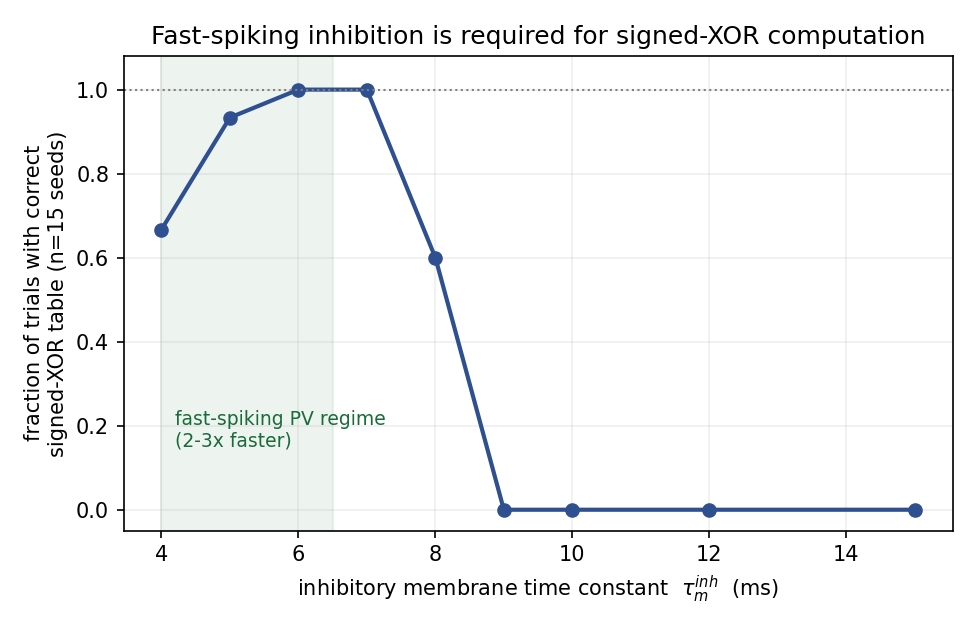
\includegraphics[width=0.78\textwidth]{exp2_pv_sweep.png}
\caption{Truth-table success rate (15 noisy seeds per point) as a function of
the inhibitory pivot's membrane time constant. The functional window
($100\%$ success) is confined to the fast-spiking, parvalbumin-like regime
($\tau_m \leq 7$~ms); the computation collapses at pyramidal and
Sst/Htr3a-like time constants.}
\label{fig:spiking_pv}
\end{figure}

This turns the firing-rate caveat of the Abstract and Section~\ref{sec:scope}
into a sharp, testable claim. The structural analysis is cell-type-agnostic
about which inhibitory subtype occupies the pivot; the dynamics are not.

\begin{prediction}{Fast-spiking pivot requirement}{pv}
A signed-XOR motif instance is \emph{functional} (computes the exclusive-or and
its signed error) only if its inhibitory pivot is a fast-spiking,
parvalbumin-type interneuron. Motif instances whose pivot is a somatostatin- or
Htr3a/VIP-type interneuron are structurally present but functionally inert
under realistic membrane time constants. Equivalently: the functional density
of the motif in cortex is bounded above by the density of \emph{PV-pivoted}
instances, which can be substantially lower than the structural density counted
on the static graph.
\end{prediction}

This prediction is directly falsifiable, both \emph{in silico} (a full
cell-type-resolved spiking simulation of the Allen V1 model should find error-
correlated activity concentrated on PV-pivoted instances) and \emph{in vivo}
(optogenetic silencing of PV vs.\ Sst interneurons should differentially
abolish mismatch responses in candidate motif circuits). It also refines the
structural counts of Section~\ref{sec:weight_stats}: the i4Pvalb dominance
observed at the stricter weight threshold $|w|\geq 1.0$ is, on this account,
the functionally relevant population, while the Sst-pivoted instances dominant
at $|w|\geq 0.1$ may be structural background.

\subsection{Result 3: the error signal is graded and correctly signed}
\label{sec:spiking_graded}

Finally we tested the graded regime of Section~\ref{sec:dynamic}. Holding the
``target'' input fixed and sweeping the ``prediction'' input from $0$ to
$1.6\times$ its level, $F^+$ fires at a fixed rate on the entire under-shoot
side (prediction below target) and falls silent once the prediction reaches the
target, while $F^-$ is silent on the under-shoot side and activates on the
over-shoot side (Figure~\ref{fig:spiking_graded}). The cross-over (minimum
error, both channels near silent) occurs at $\approx 0.9\times$ the target,
i.e.\ near match, recovering the homeostatic stopping condition. The two
channels therefore encode the sign of the mismatch with the correct polarity,
as required by the energy decomposition of Section~\ref{sec:energy}.

\begin{figure}[H]
\centering
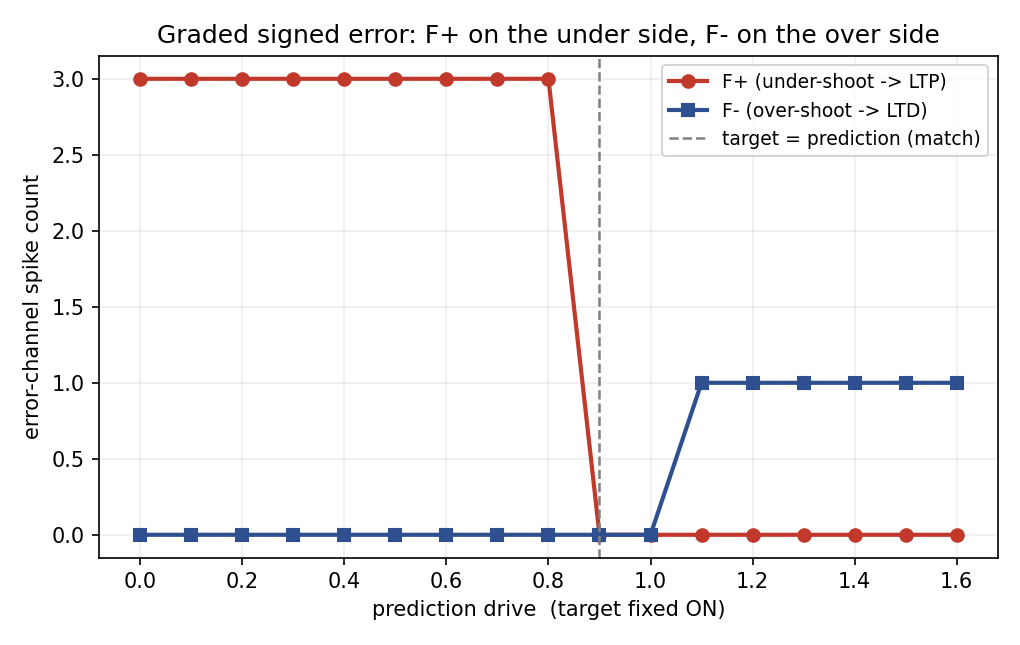
\includegraphics[width=0.78\textwidth]{exp3_graded_error.png}
\caption{Graded signed error. With the target fixed, $F^+$ (potentiation
driver) is active when the prediction under-shoots the target and $F^-$
(depression driver) is active when it over-shoots, with a near-silent
cross-over at match. The motif reads out the sign of the prediction error
without any global computation.}
\label{fig:spiking_graded}
\end{figure}

\subsection{Scope and limitations of the spiking validation}
\label{sec:spiking_scope}

\begin{remark}
This is a functional validation of the \emph{isolated} eight-neuron motif, not
of V1. It uses one neuron per role, current-based LIF dynamics with cell-type
membrane time constants, and hand-set synaptic weights; it does not include
plasticity (STDP), dendritic nonlinearities, conductance-based synapses,
short-term depression, or the recurrent embedding of the motif in the full
V1 graph. It therefore establishes that the signed-XOR computation is
\emph{realisable} in spiking dynamics with biologically plausible time
constants, and that this realisability is contingent on fast-spiking
inhibition --- but it does not establish that any particular V1 instance is
actually used this way \emph{in vivo}. Embedding the validated motif in the
Allen V1 reservoir, with cell-type-specific rates and STDP, is the natural
next step and is listed below.
\end{remark}

% --- New item for the validation plan in Section~\ref{sec:experiments} ---
% Insert the following \item into the enumerate in
% "Proposed experimental validation plan", e.g. as a new item 11.
%
% \item \textbf{Spiking functional validation (DONE, this paper,
%   \S\ref{sec:spiking}):} The isolated eight-neuron motif was simulated as a
%   cell-type-parameterised LIF network in Brian2. It reproduces the signed-XOR
%   truth table deterministically ($88\%$ under Poisson noise), produces a
%   correctly-signed graded error, and is functional \emph{only} with a
%   fast-spiking PV-type pivot ($\tau_m \leq 7$~ms; $0\%$ success at Sst/pyramidal
%   time constants), yielding the falsifiable Prediction~\ref{pred:pv}. Embedding
%   the validated motif in the full V1 reservoir with STDP remains follow-up work.

% --- Bibliography entry for Brian2 (paste into thebibliography, alpha order) ---
%
% \bibitem[Stimberg et~al., 2019]{Stimberg2019}
% Stimberg, M., Brette, R., and Goodman, D.~F.~M. (2019).
% \newblock Brian 2, an intuitive and efficient neural simulator.
% \newblock \emph{eLife}, 8:e47314.
%
% --- Optional addition to the Code and data availability section ---
%
% The spiking functional validation (Brian2/Python, \S\ref{sec:spiking}) is
% released as a standalone, MIT-licensed repository at
% \url{https://github.com/OWNER/signed-xor-motif-validation}; all figures and
% tables in this section are reproduced by a single \texttt{run\_all.py} script.
